\documentclass[a4paper]{article}
\usepackage[a4paper, total={5in, 6.5in}]{geometry}
\usepackage{color}
\usepackage{tikz}
\usepackage{lipsum}
\usepackage{geometry}
\geometry{a4paper, left=2.5cm, top=2.5cm, bottom=2.5cm, right=2.5cm}
\usepackage{changepage}
\usepackage{booktabs}
%\usepackage[labelfont = sc]{caption}
\usepackage[font=small]{caption}
\DeclareCaptionFormat{mycaptionfont}{\fontsize{12}{13}\selectfont#1#2#3}
\usepackage{threeparttable}
\usepackage{graphicx}
\usepackage{ntheorem}
\usepackage{caption}
\usepackage{wrapfig,lipsum,booktabs}

\usepackage{pdflscape}


\captionsetup{format=mycaptionfont}
\usepackage{subcaption}
\theoremseparator{:}
\usepackage{lscape}


\newtheorem{hyp}{Hypothesis}
\usetikzlibrary{shapes,decorations,arrows,calc,arrows.meta,fit,positioning}
\tikzset{
    -Latex,auto,node distance =1 cm and 1 cm,semithick,
    state/.style ={ellipse, draw, minimum width = 0.7 cm},
    point/.style = {circle, draw, inner sep=0.04cm,fill,node contents={}},
    bidirected/.style={Latex-Latex,dashed},
    el/.style = {inner sep=2pt, align=left, sloped}
}





\begin{document}
\section{Data Prep, EDA, and Theory development}
\subsection{Varaible Selection \& Explanation}
For the purpoase of analyzing the determinants of prices of home sales in the US, the followign variables were included in the analysis (Table 1): 


\begin{itemize}
  \item Sale Price (DV)
  \item Total Living Space (IV) \& Years Since Remodeling (at point of Sale) (IV)
  \item Confounders \& Controls: Quality, Lot Area, Condition
\end{itemize}



A total of 1,460 house sales were recorded between 2006 and 2010 for the district of Ames, Iowa (USA).
%\footnote{https : //www.kaggle.com/competitions/home − data − f or − ml − course/data} The dependent varibale was identified to be SalePrice. 
As can be observed in Table 1, the mean sale price of a house was (in 1000s) \$180.921 ($SD$ = 79.443). Combined with the range [34,900, 755,000], and the median ($median$ = 163.000), a positive skewness was observed ($skew$ = 1.881), i.a. suggested by this variable being a of financial nature. The Total Living Area per property displays a mean of 2,572.89 square feet (SD = 823.598) in addition to a large range of values[334, 11,752], thereby displaying a reasonably strong positive skeweness ($skew$ = 1.776).  
Years Since Remodeling (at time of sale) shows that the average property did not undergo renovations for 22.95 (~23) years ($SD$ = 20.950).\footnote{This variable was constructed by deducting the Year of Sale by Year of Last Remodelling or Building Completion} This varaible distributes reasonably constant across its data range, stopping out at a maximum of 60 years (See Figure 1B - quantiles).
Furthermore, the variable Quality represents a rating from 1 to 10, similar to a Likert Scale. Quality has to be considered a categorical variable in this case i.a. because the distances between each rating level are not constant and the distribution is skewed \textbf{(SEE SUPPLEMENTARY APPENDIX REGRESSION AND PICTURE)}. However, it was decided to include this variable in the table to display that certain statistics, such as the meam (= 6.099) and standard deviation (1.383) might warrant its treatment as a quantitative variable under certain assumptions. Noting this, the fact that Quality is a categorical variable will, thus, be relaxed in part 5 for demonstrative purposes. Finally, i.a. Lot Area will be used as a control variable in the regressions to control for the association larger lot sizes creating larger houses ($mean$ = 10516.830, $SD$ = 9981.265). 




% Table created by stargazer v.5.2.3 by Marek Hlavac, Social Policy Institute. E-mail: marek.hlavac at gmail.com
% Date and time: Wed, Sep 14, 2022 - 15:53:27
\begin{table}[!htbp] 
\begin{adjustwidth}{-0cm}{-0cm}
\begin{threeparttable}
\small
\captionsetup{font=small, justification=raggedright,singlelinecheck=false}
\caption{\textsc{Descriptive Statistics of Numeric Varaibles}}
\centering 
  \label{}   
\begin{tabular}{@{\extracolsep{1pt}}lccccccc} 
\\[-5ex]\hline 
\hline \\[-1.8ex] 
Statistic & \multicolumn{1}{c}{Mean} & \multicolumn{1}{c}{St. Dev.} & \multicolumn{1}{c}{Min} & \multicolumn{1}{c}{Pctl(25)} & \multicolumn{1}{c}{Median} & \multicolumn{1}{c}{Pctl(75)} & \multicolumn{1}{c}{Max} \\ 
\hline \\[-1.8ex] 
SalePrice & 180.921 & 79.443 & 34.900 & 129.975 & 163.000 & 214.000 & 755.000 \\ 
Lot Area & 10,516.830 & 9,981.265 & 1,300 & 7,553.5 & 9,478.5 & 11,601.5 & 215,245 \\ 
Quality & 6.099 & 1.383 & 1 & 5 & 6 & 7 & 10 \\ 
Total Living Space & 2,572.893 & 823.598 & 334 & 2,014 & 2,479 & 3,008.5 & 11,752 \\ 
Years Since Remodeling & 22.950 & 20.641 & 0 & 4 & 14 & 41 & 60 \\ 
\hline \\[-3.5ex] 
\end{tabular} 
\begin{tablenotes}[para,flushleft]
      \small
      \item\textit{Notes:} N = 1460. Quality is technically to be considered a categorical variable
    \end{tablenotes}
\end{threeparttable}
\end{adjustwidth}
\end{table}


Additionally, there are multiple categorical variables used in this assignmnent \textbf{(see Appendix)}, such as Zoning and Year of Sale. The original (MS)Zoning variable contains seven categories, of which five contain data; these zones correspond to the administrative classification of the ground on which the properties are constructed (Commercial, Floating Village, Low-Density, Moderate-Density, High-Density contain data; Residential Low Density Park, Agriculutural, Industrial do not contain records). For the purpose of this analysis, this number was reduced to four categories based on the similar behaviour of Moderate and High Density properties \textbf{(SEE SUPLEMENTARY APPENDIX PLOT)} in  the data. This is interesting as Ames, Iowa, represents the steretypical picture of a mid-western town in the US, displaying fewer densly populated areas; curtailing possibilities of extrapolation to similar samples. Thus, the main question of this analysis section focuses on the difference between Low and higher density properties.\footnote{Floating Village and Commercial behave too differently to be merged} In addition, year of sale will be used to control for the effect of the 2008/2009 housing cricis. 
% FIGURE 
\begin{figure}
\begin{adjustwidth}{-2cm}{-2cm}
\centering
\begin{subfigure}{.4\textwidth}
    \centering
    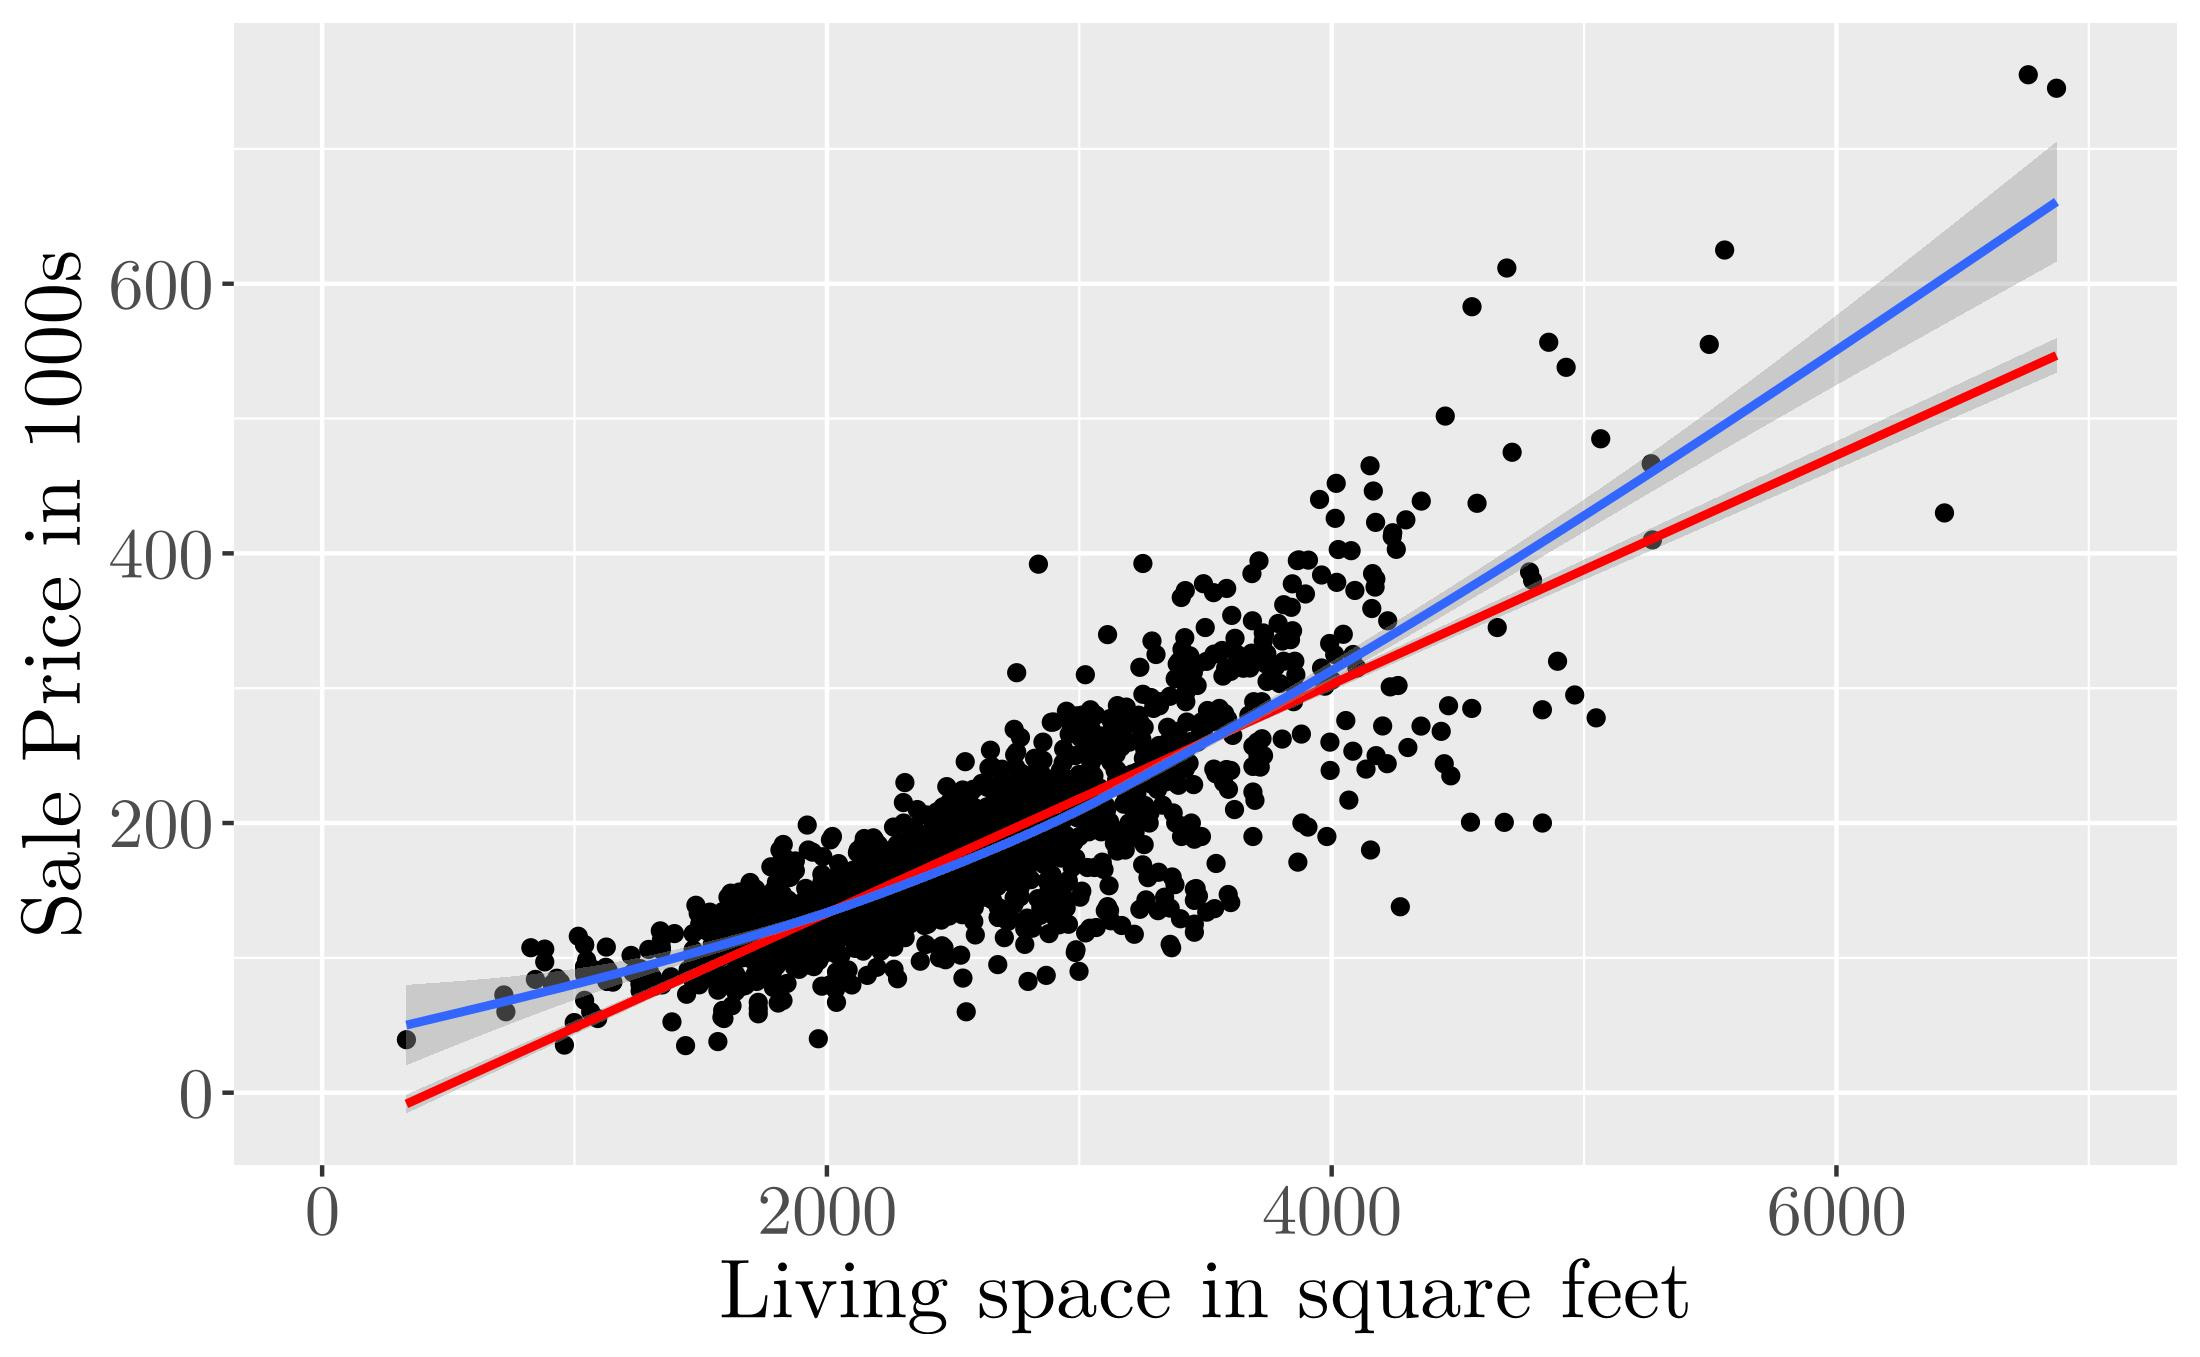
\includegraphics[width=.95\linewidth]{"/home/angelo/Documents/Uni/Courses/Advanced Statistics and programming/Assignments/assignment1/Code/h1.jpg"}  
    \caption{Positive association of total Living Space \& Sale Price; range [0, 7000]}
    \label{SUBFIGURE LABEL 1}
\end{subfigure}
\begin{subfigure}{.4\textwidth}
    \centering
    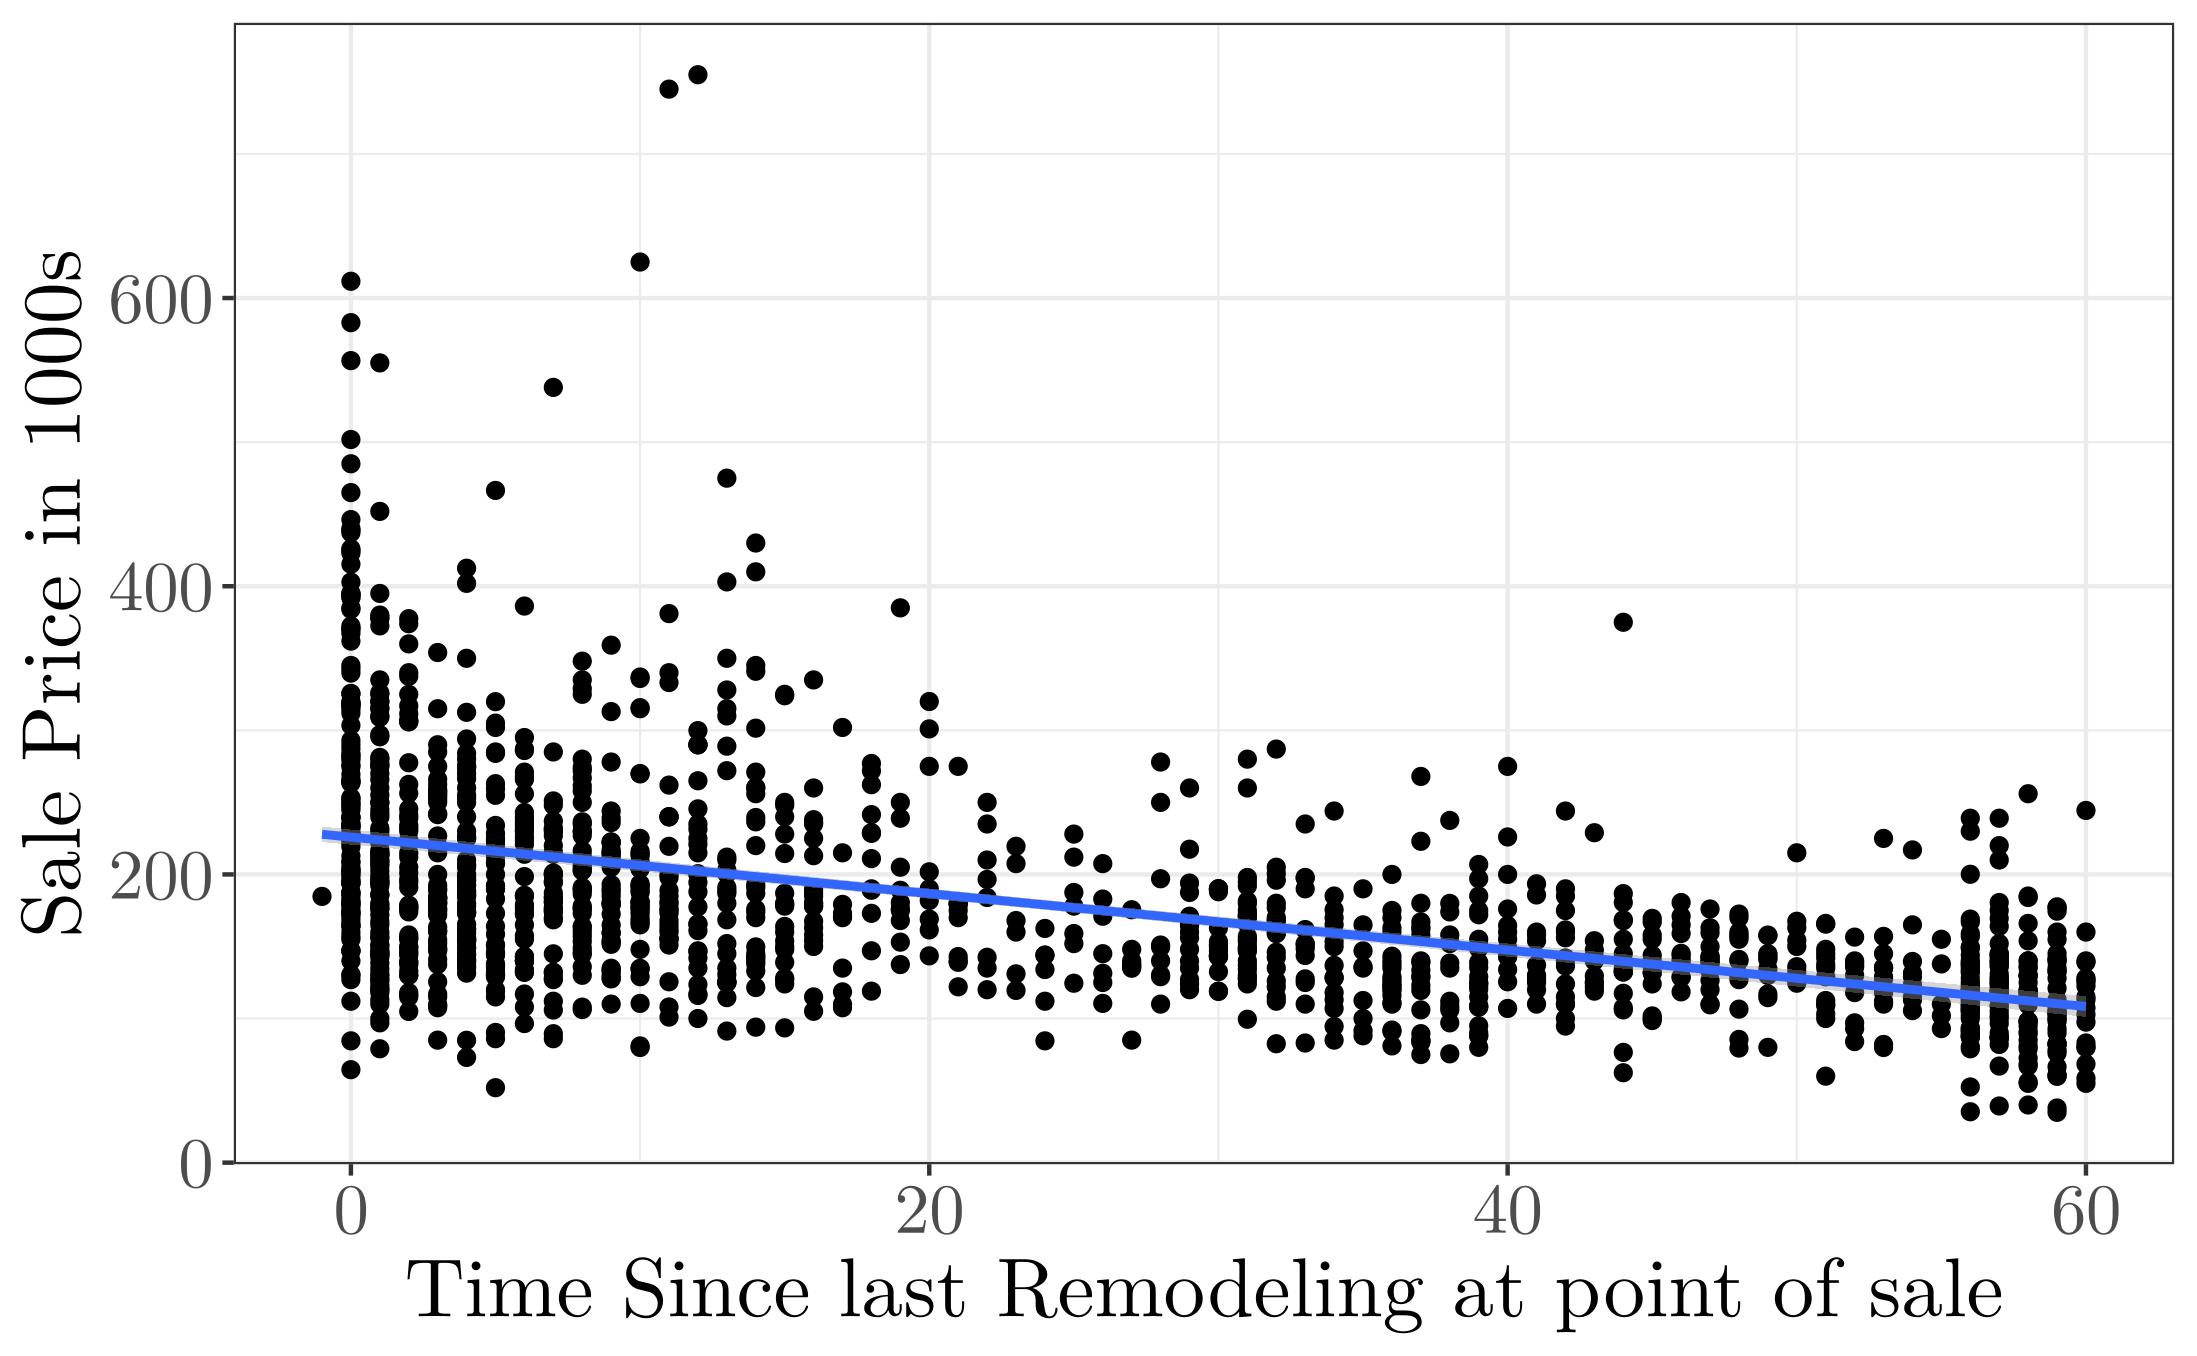
\includegraphics[width=.95\linewidth]{"/home/angelo/Documents/Uni/Courses/Advanced Statistics and programming/Assignments/assignment1/Code/h3.jpg"}  
    \caption{Negative association of Time Since Remodelling \& Sale Price}
    \label{SUBFIGURE LABEL 2}
\end{subfigure}
\begin{subfigure}{.4\textwidth}
    \centering
    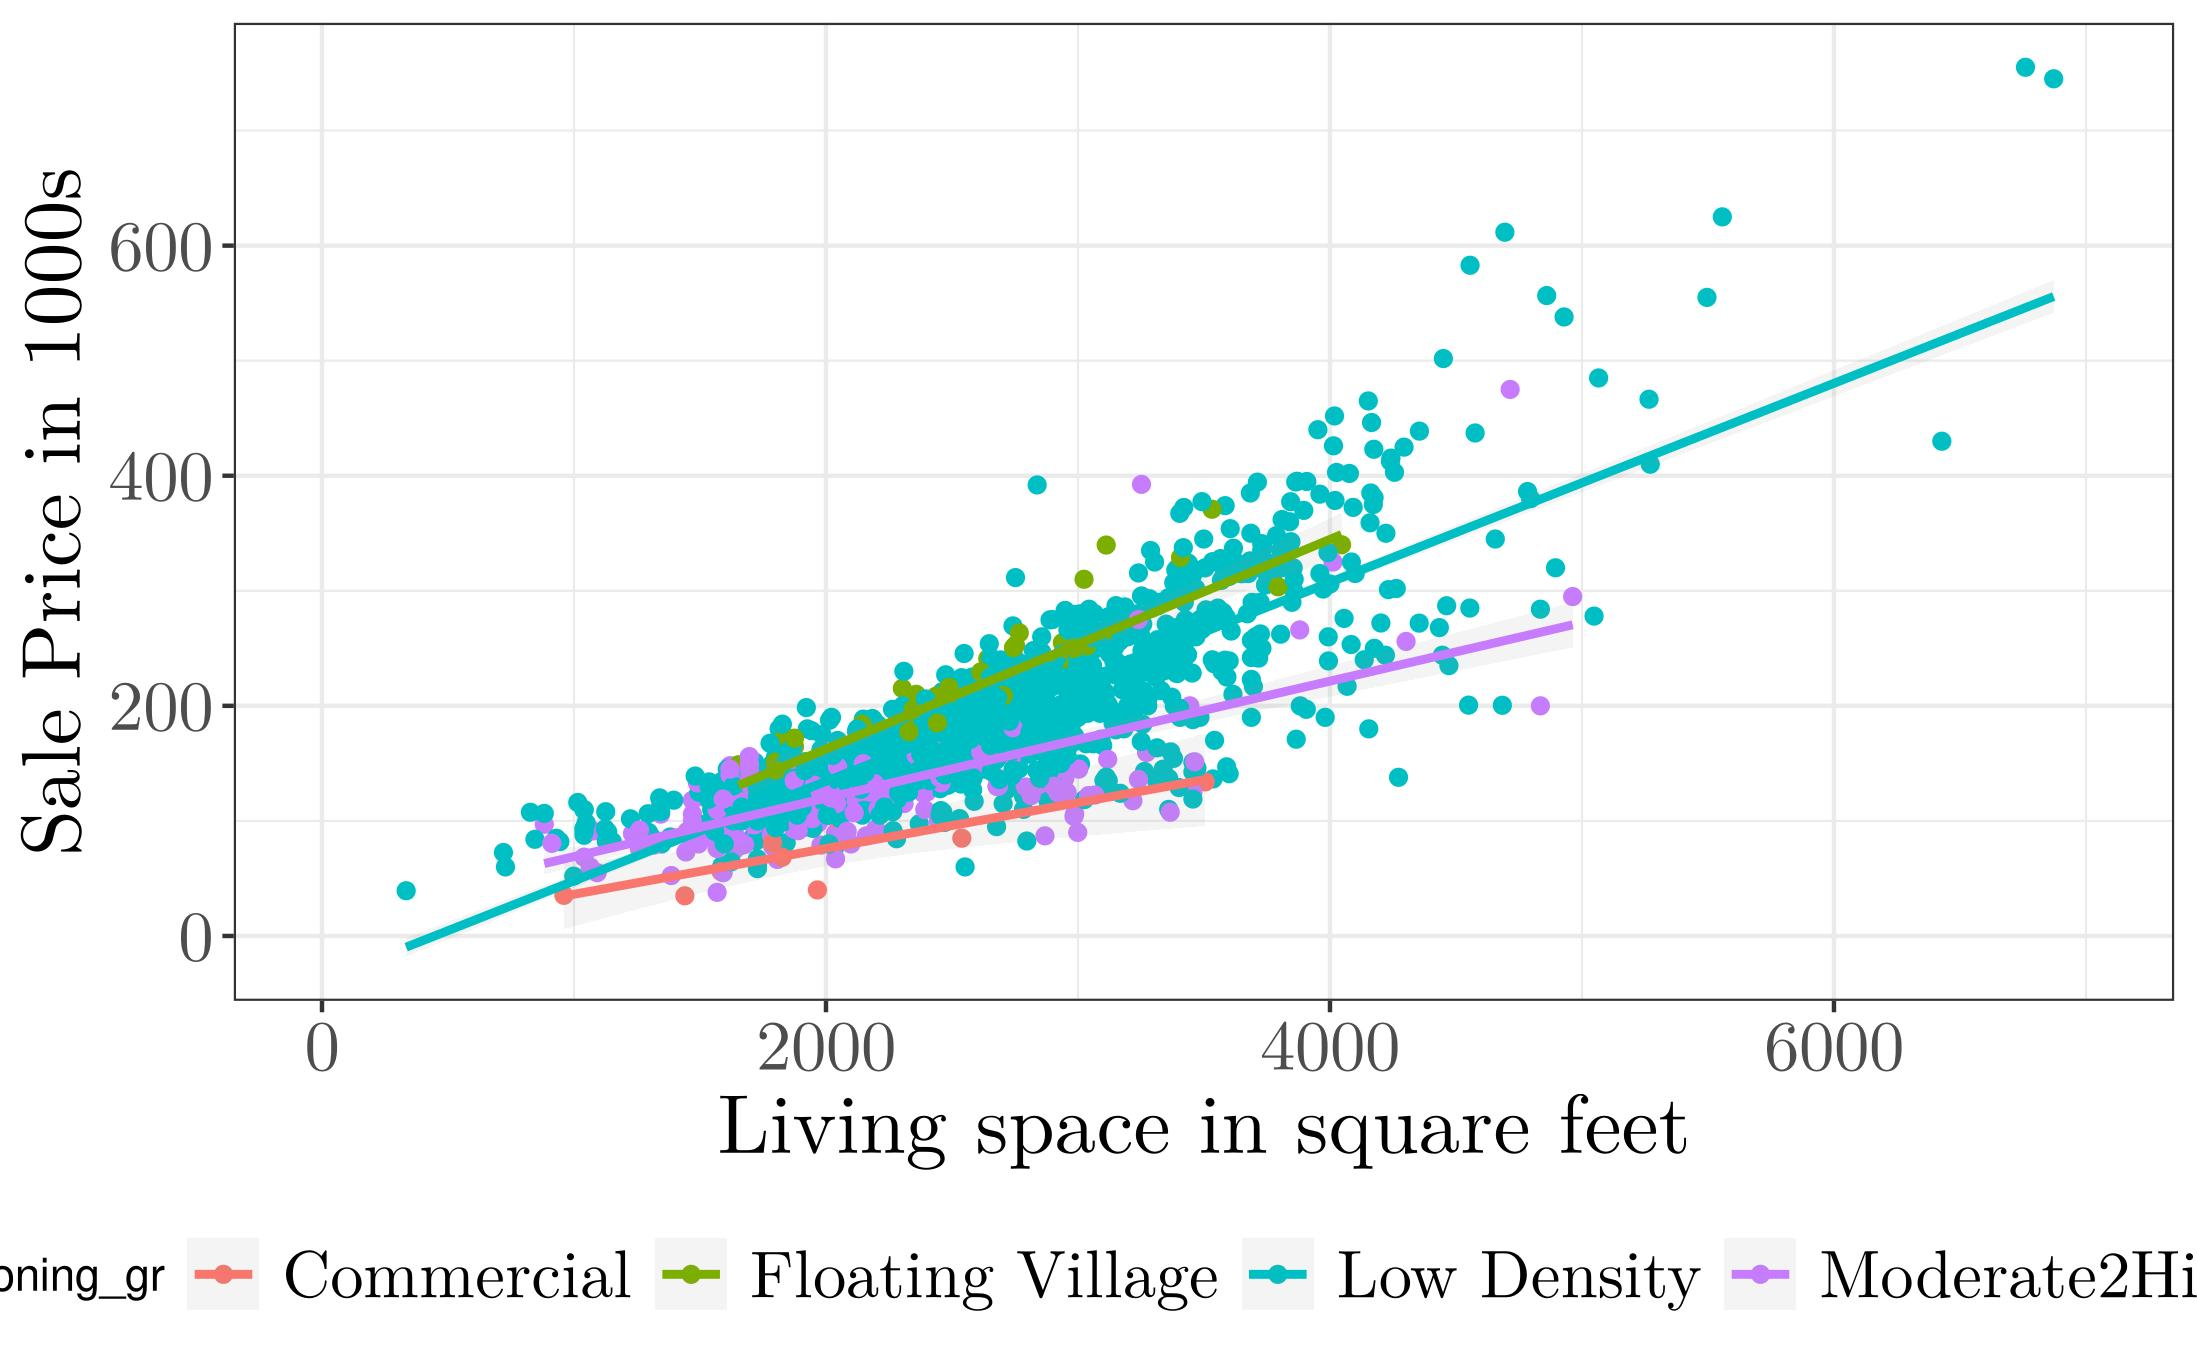
\includegraphics[width=.95\linewidth]{"/home/angelo/Documents/Uni/Courses/Advanced Statistics and programming/Assignments/assignment1/Code/h2.2.jpg"}  
    \caption{Positive association of total Living Space \& Sale Price subsectioned by Zoning}
    \label{SUBFIGURE LABEL 3}
\end{subfigure}
\small
\caption{Three Hypothesis Graphs displaying their repective association with the outcome variable}
\label{FIGURE LABEL}
\end{adjustwidth}
\end{figure}

Finally, the plots oin Figure 1 will be considered in the context of the hypotheseses set up in part 2. 



\section{Theoretical model and OLS assumptions}
\subsection{Hypotheses}
Based on the plots generated during the EDA, a mini theory was created to explain the variation in the sales price of properties (Figure 2). The primary parts of this theory invlove Total Living Space, the correspondign Zoning of the proptery, and Years Since remodleing (at point of sale). The resulting causal scheme can be seen in Figure 2. Please note, that this scheme was created in adherence to the graph theory by \textbf{cite the eci book}; thus, interaction effects are represented by direct effects between the regressors.




Based on this model, the following three hypothesis were created. 
\subsubsection{Hypotheses 1}

\begin{center}
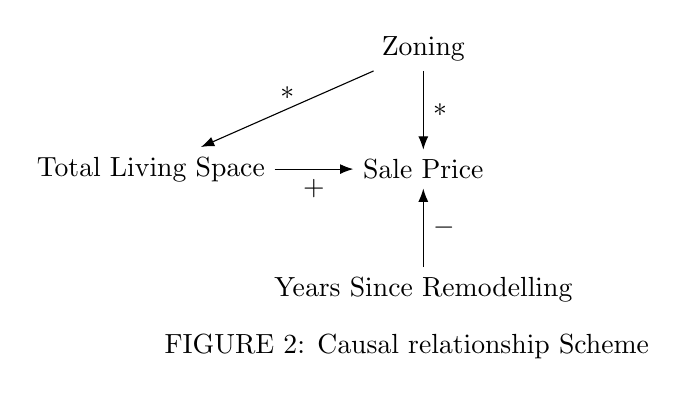
\begin{tikzpicture}
	\centering
 	\node at (3.25,-2.25) {FIGURE 2: Causal relationship Scheme};
    \node (1) at (0,0) {Total Living Space};
	\node (2) [right = of 1] {Sale Price};
	\node (3) [above = of 2] {Zoning};
	\node (4) [below = of 2] {Years Since Remodelling};

	\path (1) edge node[below] {$+$} (2);
	\path (3) edge node[right] {$*$} (2);
	\path (3) edge node[above] {$*$} (1);
	\path (4) edge node[right] {$-$} (2);
	
\end{tikzpicture}
\end{center}

\indent \textbf{Figure 1A} displays a potential direct positive association between Total Living Space (IV) and Sale Price (DV)\footnote{Including an optimally fitted line, showing potential problems of a non-linear relationship}. Thus, one expects that larger houses have a higher sale price. Consequently,this research asserts that:

\begin{hyp}[H\ref{hyp:first}] \label{hyp:first}
Total living space (IV) has a direct postive association with Sales Price (DV)
\end{hyp}


\indent Subsequently, when taking the Zoning (MSZoning or MSZoning\_grouped - IV) into account to reflect the administrative borderrs of Ames' districts, larger houses in more densly populated areas of the city appear to have a lower price when compared to houses of same size in less densly populated areas as can be seen in Figure 1c. This suggests a separation between "downtown less affluent areas" and "sub-urban affluent areas". Dditionally, the effect of Total Living Area appears to be stronger for Low Denstiy zones, which can be seen at the steeper OLS fitted line for Low Denstiy properties when compared to Moderate-to-high density properties. Thus, the second hypothesis asserts that

\begin{hyp}[H\ref{hyp:second}] \label{hyp:second}
Zoning moderates (MIV) the direct postive association of Total Living Space (IV) and Sale Price (DV). The association of Space and Sale Price is proposed to be weaker for more densly populated areas than for more rural areas. 
\end{hyp}



\indent Finally, Figure 1c shows that properties that are older or have not been remodelled more recently, tend to have a lower sale price than newer or more modern houses.Thus, the final hypothesis assserts that Years Since Remodelling display a negative effect on Sale Price; or formally:



\begin{hyp}[H\ref{hyp:third}] \label{hyp:third}
Years Since Remodeling (IV) has a negative effect on Sale Price (DV).
\end{hyp}

The resulting population regression equation based on Figure 2 is, thus, formally expressed as:

%$$ {SalePrice} = \alpha + \beta_{1} TotLivingSpace - \beta_{2}  TotLivingSpace^2 + \beta_{3}  Quality + \beta_{4}  Zoning_{Low Density} + \beta_{5}  Zoning_{Other} + \beta_{6}  YearsSinceRemodeling + \beta_{7}  LotArea + \beta_{8} TotLivingSpace*Zoning_{Low Density} + \beta_{9} TotLivingSpace*Zoning_{Other} +\epsilon$$


$$ (2-1)   \\\   {SalePrice} = \alpha + \beta_{1} Total Living Area
 + \beta_{2}  Zoning - \beta_{3}  Years Since Remodeling +\epsilon$$

It is notable, that the categorical variable Zoning will be specified as a dummy variable. Additionally, Total Living Area will also be addresseed using a quadratic function to address issues with non linearity. 

\subsection{Assumptions}

\indent A1: The linearity of model parameters and error term assumption suggests that the functional form of the underlying population regression model is linear and additive. Thus, this assumption is generally assumed to hold, i.a. not having introduced quadratic or polynominal (by parameter) terms into the population regression equation (2-1). However as Figure 1b shows, there might be a quadratic, or non linear, relationship  present between Total Living Area and Sale Price. The reason why this might be the case may be that with increasion values for Total Living Area, the Sale Price increases disproportioately to a linear effect. This might induce reduced accuracy and goodness of fit to the model. This issue is generally rectified by e.g. a quadratic term in the regression equation of the variable in question.

\indent A2: Full rank assumes that no independent variable can be a linear function of other independent variables; thus, no optimal (or none at all) solution for the parameters in question can be found. This first part of the assumtion might easily be violated when not dropping a "comparative" category of a categorical varaible. However, violations of full rank might also come in the form of multicollinearity. Multicollinearity is the "almost" violation of the full rank violation as a given variable may, for isntance, be highly correlated with another given variable. Primairly, standard errors of the model become unstable to the extend that inference from the model becomes impossible. Multicollinearity is almost always present with observational data (actually making regression interesting in the first place); However, the extend is more relevant. For example might be if we included the Total Linving Space and the TotalNumberofRooms, both of which will be strongly correlated. Further tests will be conducted to probe for this assumption violation. Soluctions include the dropping (not recommended) or combining highly correlated regressors into principal components (PCA). This will be further investiaged in part 4.

A3: This assumption is referred to as mean independence (or exogeniety); assuming that the error term of the model is independent of the regressors in the model. The result of the violation of A3 might result in severe consistency issues of the estimator, biasing estimates one or the other way.
A common way, this assumption is violated is are ommitted variables or confounders. If a given variable is left out, part of the error term can be explained by a given variable which suffers under the influence of the confounder. For example, missing crime data by location explains why certain neighborhoods outperform others. This is also the reason why this varaible was left out of the mini theory. Thus, given a certain Neighborhood in question, part of the variance that would have been explained by the Crime variable is now falsely attributed to Neighborhood, biasing the estimate.

A4: The assumption of homoscedasticity assumes constant variance for the error term. However, if the variance of the estimate is varying for different observations, we face heteroscedastic variances. While this is not necessarily problematic regarding the estimated parameter (coefficient), heteroscedastictiy impacts the standard errors of the estimate, leading to problems regarding inference; (both over- and understated standard errors) potentially leading to either Type I or II error problems. In this research, this violation might occur if the eg. sales prices vary stronger for large houses than for small houses. The resulting (averaged) standard error would neither be rebresenative for small and large house standard errors and, thus, inference itself. However, this assumption becomes less relevant with large samples, particualrly for the estimate, as is the case here.

A5: Data generation: data can be the result of observational kind and random experiments. Due to the data originating from sales in a town in Iowa (Ames), we have to assume that the data is "fixed". Thus, inference regardign a wider population cannot be made from this data, as its fixed nature only applies to small towns in the mid-western USA. However, we can assume that the fixed variables collected are measured without error; particualrly as the sample collected can be somewhat representative of the wider popualtion of small towns in the mid-western USA. 

A6: If the residuals do not follow a standard normal distribution, this might result in incorrect decisions (Type I or II; both possible). This assumption is needed for performing parametric tests and generating confidence intervals. This might be the case if for instance we do not have a lot of observations for e.g. subcategories. Subsequently, the resulting inference might be biased. However, as the sample size increases, most distributions approach the normal form. 
 Nonetheless, an indication of this assumption beign violated is the presence of large amounts of outliers. As can be seen in Figure 1a the range goes from 0 to 7000 square feet, thus, ommiting two extreme observations; admittedly few in numbers. 


\section{OLS regression and model fit}
\subsection{Normal Regression}

% Table created by stargazer v.5.2.3 by Marek Hlavac, Social Policy Institute. E-mail: marek.hlavac at gmail.com
% Date and time: Wed, Sep 14, 2022 - 15:53:27
\begin{table}[!htbp] \centering 
\begin{adjustwidth}{0.cm}{-0cm}
\begin{threeparttable}
\small
\captionsetup{font=small, justification=raggedright,singlelinecheck=false}
\caption{\textsc{Non-Robust Regression Results Part 3}}
\centering 
  \label{}
\small 
\begin{tabular}{@{\extracolsep{-2pt}}lcccccc} 
\\[-5.8ex]\hline 
\hline \\[-1.8ex] 
 & \multicolumn{6}{c}{\textit{Dependent variable:}} \\ 
\cline{2-7} 
\\[-1.8ex] & \multicolumn{2}{c}{SalePrice in 1000s} & \multicolumn{2}{c}{SalePrice in 1000s} & \multicolumn{2}{c}{ln\_SalePrice  in 1000s} \\ 
\\[-1.8ex] & Model (1) & Std. Coef.& Model (2) & Std. Coef.&  Model (3) & Std. Coef.\\ 
\hline \\[-1.8ex] 
 Constant & 15.229 &  & 24.550 &  & 3.584$^{***}$ &  \\ 
  & (25.697) &  & (24.541) &  & (0.114) & \\ 
  & & & & & & \\ 
 Living Space & 0.035$^{***}$ & 0.362$^{***}$ & 0.038$^{***}$ & 0.393$^{***}$ & 0.0003$^{***}$ & 0.684$^{***}$ \\ 
  & (0.002) & & (0.005) & & (0.00002) &  \\ 
  & & & & & & \\ 
 Years Since Remodeling & $-$0.492$^{***}$ & $-$0.128$^{***}$ & $-$0.493$^{***}$ & $-$0.128$^{***}$ & $-$0.003$^{***}$ & $-$0.170$^{***}$ \\ 
  & (0.056) &  & (0.051) &  & (0.0002) &  \\ 
  & & & & & & \\ 
 Low Dens. Zone & 16.640$^{***}$ & 0.086$^{***}$ & $-$31.118$^{***}$ & $-$0.160$^{***}$ & 0.077$^{**}$ & 0.079$^{**}$ \\ 
  & (2.753) &  & (8.368) & & (0.039) &  \\ 
  & & & & & & \\ 
 Commercial Zone & $-$25.251$^{**}$ & $-$0.026$^{**}$ & $-$35.782 & $-$0.037 & $-$0.673$^{***}$ & $-$0.139$^{***}$ \\ 
  & (11.881) &  & (35.624) &  & (0.165) &  \\ 
  & & & & & & \\ 
 Floating Zone & 18.710$^{***}$ & 0.049$^{***}$ & $-$8.247 & $-$0.021 & 0.127 & 0.065 \\ 
  & (5.258) & & (22.841) & & (0.106) &  \\ 
  & & & & & & \\ 
 Lot Area & 0.001$^{***}$ & 0.074$^{***}$ & 0.005$^{***}$ & 0.616$^{***}$ & 0.00002$^{***}$ & 0.404$^{***}$ \\ 
  & (0.0001) &  & (0.0005) &  & (0.00000) &  \\ 
  & & & & & & \\ 
  
 I(Living Space$\hat{\mkern6mu}$2) &  &  & $-$0.00000 & $-$0.002 & $-$0.00000$^{***}$ & $-$0.234$^{***}$ \\ 
  &  &  & (0.00000) &  & (0.000) &  \\ 
  & & & & & & \\ 
 Living Space:Low Dens. Zone &  &  & 0.019$^{***}$ & 0.308$^{***}$ & 0.00002 & 0.058 \\ 
  &  &  & (0.004) & & (0.00002) &  \\ 
  & & & & & & \\ 
 Living Space:Commercial Zone &  &  & 0.0001 & 0.0002 & 0.0002$^{**}$ & 0.067$^{**}$ \\ 
  &  &  & (0.017) & & (0.0001) & \\ 
  & & & & & & \\ 
 Living Space:Floating Zone &  &  & 0.013 & 0.088 & 0.00002 & 0.022 \\ 
  &  &  & (0.009) &  & (0.00004) & \\ 
  & & & & & & \\ 
 Living Space:Lot Area &  &  & $-$0.00000$^{***}$ & $-$0.647$^{***}$ & $-$0.000$^{***}$ & $-$0.396$^{***}$ \\ 
  &  &  & (0.00000) &  & (0.000) &  \\ 
  & & & & & & \\ 
  Year Sold & YES & YES & YES & YES & YES & YES \\ 
  %&  & &  &  \\ 
  % & & & & \\ 
  Overall Quality Rating & YES & YES & YES & YES & YES & YES \\  
  % & (32.730) & (32.730) & (30.513) & (30.513) \\ 
  %& & & & \\ 
  Building Type & YES & YES & YES & YES & YES & YES \\ 
  %& (2.654) & (2.654) & (2.501) & (2.501) \\ 
  % & & & & \\ 
\hline \\[-1.8ex]  
\end{tabular} 
%%%%%%%
\small 
\centering
\begin{tabular}{@{\extracolsep{39pt}}lcccccc} 
R$^{2}$ && 0.803 &   0.836 &  0.861   \\ 
Adjusted R$^{2}$ && 0.800 &  0.833 &   0.858  \\ 
Residual Std. Error && 35.548  & 32.488  & 0.150   \\ 

F Statistic& & 292.393$^{***}$    & 291.609$^{***}$   & 354.941$^{***}$    \\ 

\hline 
\hline \\[-3.5ex] 
\end{tabular} 
\begin{tablenotes}[para,flushleft]
      \small
      \item\textit{Note:} N = 1460. All observations included in any model. *** p$<$0.01, ** p$<$0.05, * p$<$0.1. This table reportes the (unstandardized) regression results for the Model (1) excluding any interaction effects \& and inclduing those interaction effects in Model (3). The corresponding standardized coefficients can be foudn in Std.Model (2) \& (3). For complementary regression models \textbf{see appendix}. The comparison category in "Zone" (IV) is "Moderate-to-High Density". Years in date range is 2006 to 2010. The Sale Price is represented in 1000s.
    \end{tablenotes}
\end{threeparttable}
\end{adjustwidth}
%
\end{table}


Table 2 displays the regression results for three incrementally compelx models to explain Sale Price. These models were chosen as they concisely combine most necessary information for part 3, and 4. Standardized coefficients are adjacent to the respective models. Standard errors are not robust (see part 4). 
Overall, all three reported models are each jointly significant, displaying a significant F-test ($F$ = 292.393, $p$ $<$  0.001; $F$ = 291.609, $p$ $<$ 0.001, $F$ = 354.941, $p$ $<$  0.001). 
Not considering the control variables and interaction terms, the results of model one suggest that Total Living Area have a signifiacnt positive effect on Sale Price ($\hat{\beta}$ = 0.035, $p$ < 0.001) as hypothesized. Thus, an increase in Living Area by one square feet increases the sale price by \$35\footnote{remember: Sale Price is in 1000s}.
Additionally, Years Since Remodeling follows the expected pattern and shows a significant negative effect on Sale Price ($\hat{\beta}$ = -0.492, $p$ $<$ 0.001). Additionally, when compared to the Moderate to High category in Zoning, the Low Density Zone shows a signifiacnt higher Sale Price (intercept) ($\hat{\beta}$ = 0.086, $p$ $<$ 0.001). Finally, this model explains 80.3\% of the variation in Sale Price.

\indent Now considering model (2), which includes several interaction terms and one quadratic term.\footnote{Note: model (3) will be used in part 4} We see that the coefficeints for Living Space ($\hat{\beta}$ = 0.038, $p$ $<$ 0.001) and Years Since Remodelling ($\hat{\beta}$ = -0.493, $p$ $<$ 0.001) display almost no changes. Furthermore, the interesing interaction terms report significant findings. Primairly, the Low Density Zone seems to disply a stronger positve relationship in terms of Living Space and Sale Price when compared to hig to Medium density zone ($\hat{\beta}$ = -0.308, $p$ $<$ 0.001). Furthermore, the quadratic term of Living Space is significant, suggesting an increase of Sale Price veyond the linear term expressed above ($\hat{\beta}$ = -0.002, $p$ $<$ 0.01). however, what is most striking about the model is that the Low Density Zone appears to change its direction; when compared to the Moderate to High Density Zone, the Low density Zone reports a lower Sale Price. It might be noted, that part of this might be explained by the interaction of Living Space and Low Density Zone ($\hat{\beta}$ = 0.019, $p$ $<$ 0.001), which still shows, that there might be a positive relationship between Living Space and Sale Price hypothesized to be higher for Low Density (see next section).

Finally, the model (2) improved significantly in model fit over the model (1) significantly beyond chance, reported by $adjR²$. As such not only the model (2) ($R²$ = 0.836,$adjR²$ = 0.833) improved the model fit significantly over model (1) ($R²$ = 0.803,$adjR²$ = 0.800). Thus, the inclusion of the interaction terms improved on the model.

\subsection{Standardized coeffiicents}
However, while the evaluation of the fit of the models can be done via $adjR²$, the comparions of the regressors is not directly possible. this is due to the difference in ranges for the data. Subsequently, Table 2 reports the standardized coefficietnts adjacent to the unstandardized coefficients. Overall, when ignoreing the control variable (model (2)) Lot Area ($\hat{\beta}std$ = 0.616, $p$ $<$ 0.001), of the theory relevant variables, it might appear that Living Space dispalys the larges effect Size ($\hat{\beta}std$ = -0.393, $p$ $<$ 0.001). This is also in accordance with model (1). However, becasue of this specific reason, the control variable Lot area, and its interaction with Living Space was included, as it displays a very large standardizeed negative term ($\hat{\beta}std$ = -0.647, $p$ $<$ 0.001). Thus, while it might appear from the standardized coefficients, that Living Space has the largest effect size, it is notable that Years Since Remodeling ($\hat{\beta}adj$ = -0.128, $p$ $<$ 0.001) has a larger effect size than Living Space. Finally, the standardized coefficient for the interaction of Living Space and Low Density Zone $\hat{\beta}adj$ = 0.308, $p$ $<$ 0.001) now exceeds the negative std. coefficient for Low Density Zone $\hat{\beta}adj$ = -0.160, $p$ $<$ 0.001), suggesting support for hypothesis (2) after all. \footnote{Please note that the interpretation of effect sizes follows that if eg. X changes by one standard deviation, how many standard deviations does the outcome change. This is uninformatiove, and, thus, not reported}
To conclude, among the quantitative relevant variables, the largest effect size should be attributed to Years Since Remodelling, ignoring control variables, due to the aboforementioned interaction term. 



\section{Diagnostic checking}
\subsection{A1}
As can be seen in Figure 1a, Total Living Space tends to display non linearity with the outcome. Subsequently, Table 2 shows the inclusion of a quadratic term when compraing Model 2 and 3. Overall, including not only the qudratic term ($\hat{\beta}$ = 0.002, $p$ $<$ 0.001; $adj.\hat{\beta}$ = 0.234, $p$ $<$	 0.001), but also logscaling the outcome improves the model beyond chance. Thus, the issue of non-linearity is reduced.


\subsection{A2}

\begin{table}[!htbp] \centering 
\begin{adjustwidth}{0.5cm}{-0cm}
\begin{threeparttable}
\small
\captionsetup{font=small, justification=raggedright,singlelinecheck=false}
\caption{\textsc{VIF reports }}
\centering 
  \label{}
\small 
\begin{tabular}{@{\extracolsep{-7pt}}lcccccc} 
\\[-5.8ex]\hline 

 & GVIF & Df & GVIF$\hat{\mkern6mu}$(1/(2\textasteriskcentered Df)) \\ 
\hline \\[-1.8ex] 
tot\_liv\_area & $22.682$ & $1$ & $4.763$ \\ 
y\_since\_rem & $1.535$ & $1$ & $1.239$ \\ 
low\_density\_zone & $16.161$ & $1$ & $4.020$ \\ 
commercial\_zone & $11.942$ & $1$ & $3.456$ \\ 
floating\_zone & $30.700$ & $1$ & $5.541$ \\ 
I(tot\_liv\_area$\hat{\mkern6mu}$2) & $31.756$ & $1$ & $5.635$ \\ 
LotArea & $32.949$ & $1$ & $5.740$ \\ 
YrSold & $1.051$ & $4$ & $1.006$ \\ 
OverallQual\_cat & $4.301$ & $9$ & $1.084$ \\ 
Building\_type & $1.189$ & $1$ & $1.090$ \\ 
tot\_liv\_area:low\_density\_zone & $31.262$ & $1$ & $5.591$ \\ 
tot\_liv\_area:commercial\_zone & $11.544$ & $1$ & $3.398$ \\ 
tot\_liv\_area:floating\_zone & $31.772$ & $1$ & $5.637$ \\ 
tot\_liv\_area:LotArea & $46.292$ & $1$ & $6.804$ \\ 
 
\hline \\[-3.5ex] 
\end{tabular} 
\begin{tablenotes}[para,flushleft]
      \small
      \item\textit{Note:} N = 1460. 
    \end{tablenotes}
\end{threeparttable}
\end{adjustwidth}
%
\end{table}
Considering multicollinearity, Table 3 reports the VIF for the variables in the main model (3) (see Table 2) excluding control-categorical variables. In order to assess multicollinearity, the VIF was calculated. To make the resulting VIF comparable, the GVIF\^(1/(2*Df)) is used.\footnote{\textbf{IMPORTANT %$https://www.tandfonline.com/doi/abs/10.1080/01621459.1992.10475190#.U2jkTFdMzTo$
}} While some variables display a VIF of more than 5, this does not automatically suggest multicollinearity. However, this necessitates further anaylysis. Considering i.a. Table 2 again, one can see that the standard errors remain stable across all models\footnote{(not reported) There seems to be some multicollinearity problems with the control variable categories of Quality}. The inclusion of more varibles, interaction terms, or scaling the outcome, does not cause the standard error estimates to vary considerably. Finally, the stability of the model and the significane of most of the terms in context of the significanfce of the overall model ($F$ = 354.941, $df$ = 25) indicates that multicollinearity might not pose a considerable problem in this model.

\subsection{A4}
Table 4 presents the regression results for model (3) in Table 2 with robust standard errors (White) in model (2) of Table 4, and clustered standard errors by Neighborhood in model (3). Neighborhood was chosen due to the assumption that houses in the same neighborhood might share variance (such as lower crime neighborhoods). Overall, this research does not seem to suffer from any systematic problems of heteroscedasitity, considering the stablity of the standard erros across all three reported model in Table 4.\footnote{Large Changes in Standrad errors in the Commercial Zone category and Floating Zone category might be attributable to their very small sample size}. Complementarily, the residulas vs fitted plot in Figure 2, in addition to the Breusch Pagan test ($BP$ = 106.62, df = 25, $p$ < 0.001), maintianing the null hypothesis of constant distributed resiudals, heteroscedasticity does not seem to pose a problem in this model. 


% FIGURE 

\begin{figure}{L}{5.5cm}
		\centering
         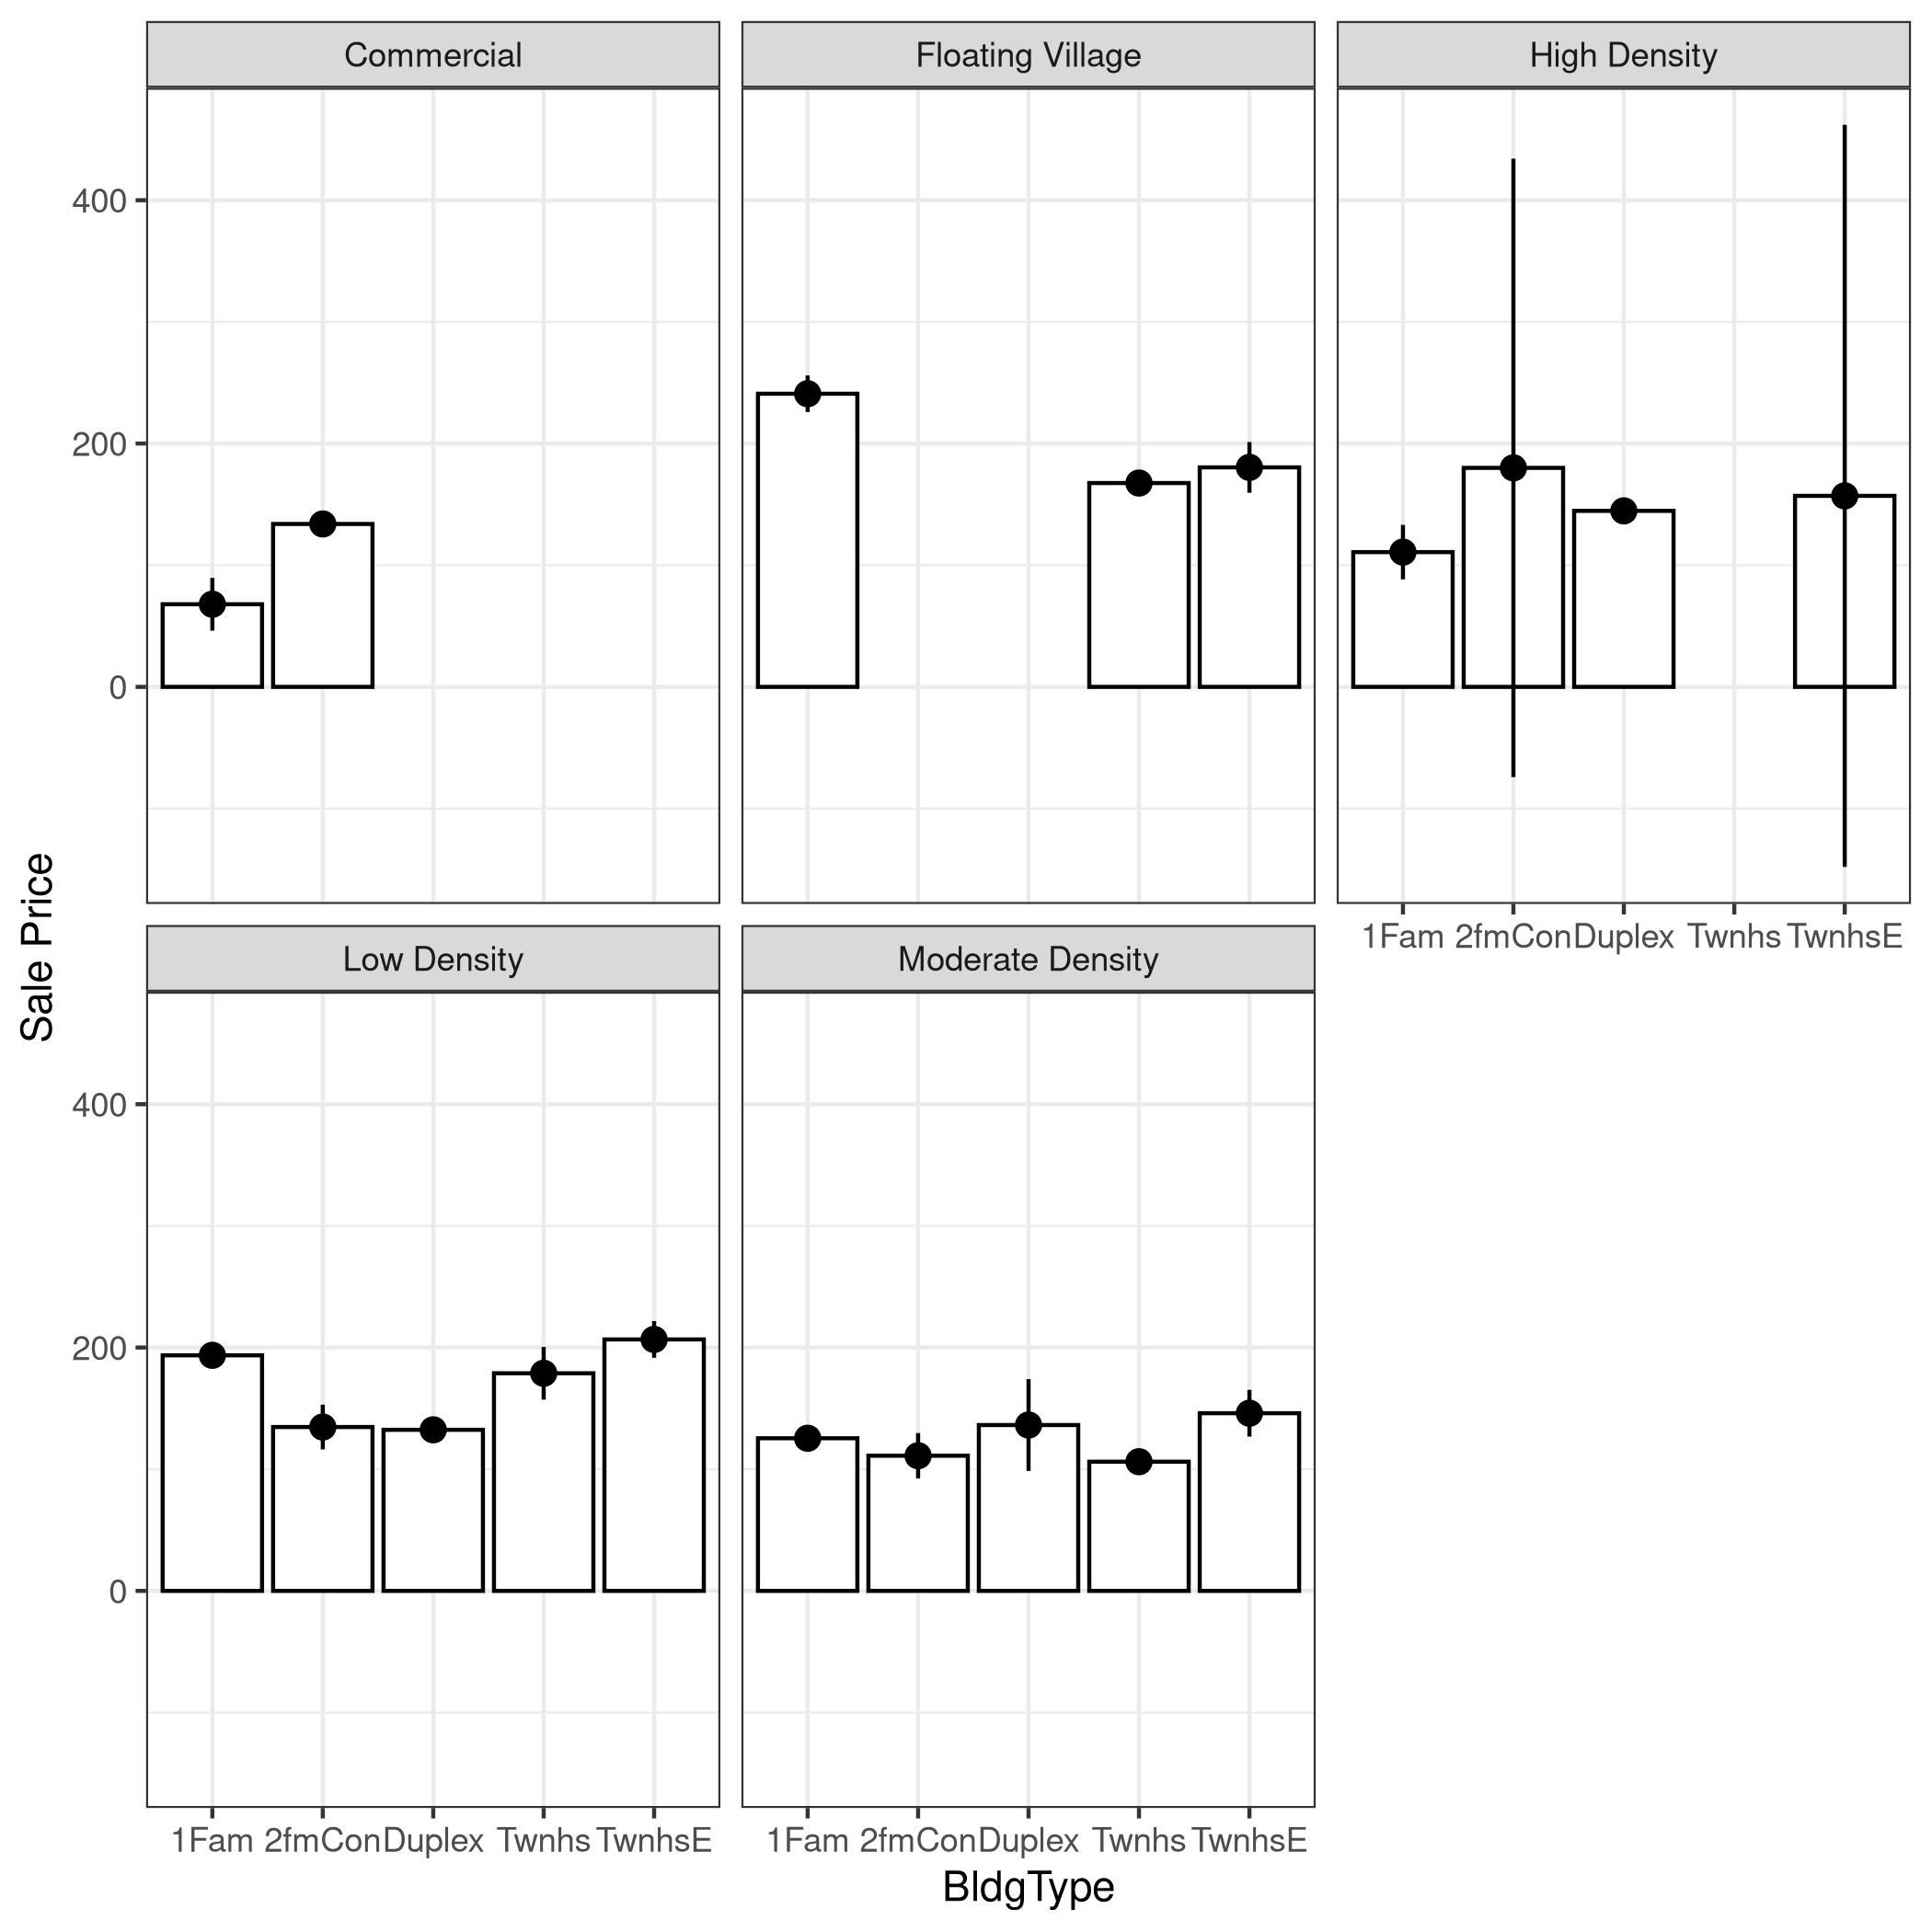
\includegraphics[scale=0.5]{"/home/angelo/Documents/Uni/Courses/Advanced Statistics and programming/Assignments/assignment1/Code/normalityplots.png"}
         \small
         \caption{Residual Distribution Plots}


\end{figure}

% Table created by stargazer v.5.2.3 by Marek Hlavac, Social Policy Institute. E-mail: marek.hlavac at gmail.com
% Date and time: Thu, Sep 15, 2022 - 23:23:18
\begin{table}[!htbp] \centering 
\begin{adjustwidth}{0.5cm}{-0cm}
\begin{threeparttable}
\small
\captionsetup{font=small, justification=raggedright,singlelinecheck=false}
\caption{\textsc{Robust OLS Regression Results}}
\centering 
  \label{}
\small 
\begin{tabular}{@{\extracolsep{-7pt}}lcccccc} 
\\[-5.8ex]\hline 
\hline \\[-1.8ex] 
 & \multicolumn{3}{c}{\textit{Dependent variable:}} \\ 
\cline{2-4} 
\\[-1.8ex] & \multicolumn{3}{c}{ln\_SalePrice} \\ 
\\[-1.8ex] & (1) & (2) & (3)\\ 
\hline \\[-1.8ex] 
 Constant & 3.584$^{***}$ & 3.584$^{***}$ & 3.584$^{***}$ \\ 
  & (0.114) & (0.048) & (0.053) \\ 
  & & & \\ 
 Living Space &  0.0003$^{***}$ & 0.0003$^{***}$ & 0.0003$^{***}$ \\ 
  & (0.00002) & (0.00003) & (0.00004) \\ 
  & & & \\ 
 Years Since Remodeling & $-$0.003$^{***}$ & $-$0.003$^{***}$ & $-$0.003$^{***}$ \\ 
  & (0.0002) & (0.0003) & (0.0003) \\ 
  & & & \\ 
 Low Density Zone & 0.077$^{**}$ & 0.077 & 0.077 \\ 
  & (0.039) & (0.047) & (0.049) \\ 
  & & & \\ 
 Commercial Zone & $-$0.673$^{***}$ & $-$0.673$^{***}$ & $-$0.673 \\ 
  & (0.165) & (0.239) & (0.490) \\ 
  & & & \\ 
 Floating Zone & 0.127 & 0.127$^{*}$ & 0.127$^{*}$ \\ 
  & (0.106) & (0.072) & (0.076) \\ 
  & & & \\ 
 I(Living Space$\hat{\mkern6mu}$2) & $-$0.00000$^{***}$ & $-$0.00000$^{***}$ & $-$0.00000$^{**}$ \\ 
  & (0.000) & (0.000) & (0.000) \\ 
  & & & \\ 
 Lot Area & 0.00002$^{***}$ & 0.00002$^{***}$ & 0.00002$^{***}$ \\ 
  & (0.00000) & (0.00000) & (0.00000) \\ 
  & & & \\  
 Living Space:Low Density Zone & 0.00002 & 0.00002 & 0.00002 \\ 
  & (0.00002) & (0.00002) & (0.00002) \\ 
  & & & \\ 
 Living Space:Commercial Zone & 0.0002$^{**}$ & 0.0002 & 0.0002 \\ 
  & (0.0001) & (0.0001) & (0.0003) \\ 
  & & & \\ 
 Living Space:Floating Zone & 0.00002 & 0.00002 & 0.00002 \\ 
  & (0.00004) & (0.00003) & (0.00003) \\ 
  & & & \\ 
 Living Space:Lot rea & $-$0.000$^{***}$ & $-$0.000$^{***}$ & $-$0.000$^{***}$ \\ 
  & (0.000) & (0.000) & (0.000) \\ 
  & & & \\ 
  Year Sold & YES & YES & YES  \\ 
  %&  & &  &  \\ 
  % & & & & \\ 
  Overall Quality Rating & YES & YES & YES  \\  
  % & (32.730) & (32.730) & (30.513) & (30.513) \\ 
  %& & & & \\ 
  Building Type & YES & YES & YES \\ 
  %& (2.654) & (2.654) & (2.501) & (2.501) \\ 
  % & & & & \\ 
\hline \\[-1.8ex] 

R$^{2}$ & 0.861 & 0.861 & 0.861 \\ 
Adjusted R$^{2}$ & 0.858 & 0.858 & 0.858 \\ 
Residual Std. Error (df = 1434) & 0.150 & 0.150 & 0.150 \\ 
F Statistic (df = 25; 1434) & 354.941$^{***}$ & 354.941$^{***}$ & 354.941$^{***}$ \\ 
\hline 
\hline \\[-3.5ex] 
\end{tabular} 
\begin{tablenotes}[para,flushleft]
      \small
      \item\textit{Note:} N = 1460. All observations included in any model. OLS estimates, robust standard errors in parentheses.*** p$<$0.01, ** p$<$0.05, * p$<$0.1. 
    \end{tablenotes}
\end{threeparttable}
\end{adjustwidth}
%
\end{table}


\subsection{A6}
Considering the $N=$ 1460 sample size, applying the Shapiro-Wilk test returns an expected rejection of non-normal distribution of the resiudals ($SW$ = 0.95161,  $p$ $<$ 0.001). Interestingly, without log scaling the Sale Price (DV) and introducing the quadratic term for Total Living Space, the normality plot in Figure 3 suggests some nonelinearity, while showing a significant Shapiro-Wilk test ($SW$ = 0.8712,  $p$ $<$ 0.001). However, this largely disappears after applying both the log scale on the outcome and the quadratic term on the Total Living Space in model (3) of Table 2 (see Figure 2 upper right). Nevertheless, due to the large sample size, issues with the normal distribution assumption of theresiudals can be neglected in this case. 



% FIGURE 
\begin{figure}

         \includegraphics[scale=0.20]{"/home/angelo/Documents/Uni/Courses/Advanced Statistics and programming/Assignments/assignment1/Code/BIGNONNORMALITYPROBLEMWITHOUTLOGSCALE"}
         \small
         \caption{Normality Plots}
\end{figure}










\section{Subset analyses}
Finally, the subset analysis considers two different models due to breviety concerns. For sake of this exercise, Qulaity will be considered a quantitative variable. additionally, assumptions regarding normaltiy and scaling are ignored for simplicity. The preceeding models show the interaction on Building type, quality and years since remodeling. 
As can be seen in Table 5, the subset analysis contains two types: the interaction of Years Since Remodelled and Overall Quality, both to be quantitaive, and Zoning, where the categories of interest are Low Density vs High Density (See Figure 1c). 
From the interpretation of Quality ($SW$ = 31.370  $p$ $<$ 0.001) and Years Since Remodelling ($SW$ = 1.890,  $p$ $<$ 0.001) as an interaction term ($SW$ = -0.418,  $p$ $<$ 0.001) follows, as expected, that for one year more not remodelled, the effect of a unit change in Quality on Sale Price is reduced by \$418. Thus, Years Since Remodeling has a negative (assumed) effect on the relationship of Quality on Sale Price. 
Following this line of thought, as was done in Part 3, the interpretation of subset analysis regarding simple categories is that  Low Density Zone properties show a \$1670 lower Sale Price than Moderate to High Density properties. Then, considering the interaction term of Living Area and Low Density Zone, this implies that given the Zone Low Density, the effect of Living Area on Sale Price is \$ 9 stronger per additional square feet in Living Area when compared to Moderate to High Density Zone.  






% FIGURE 
\begin{figure}

         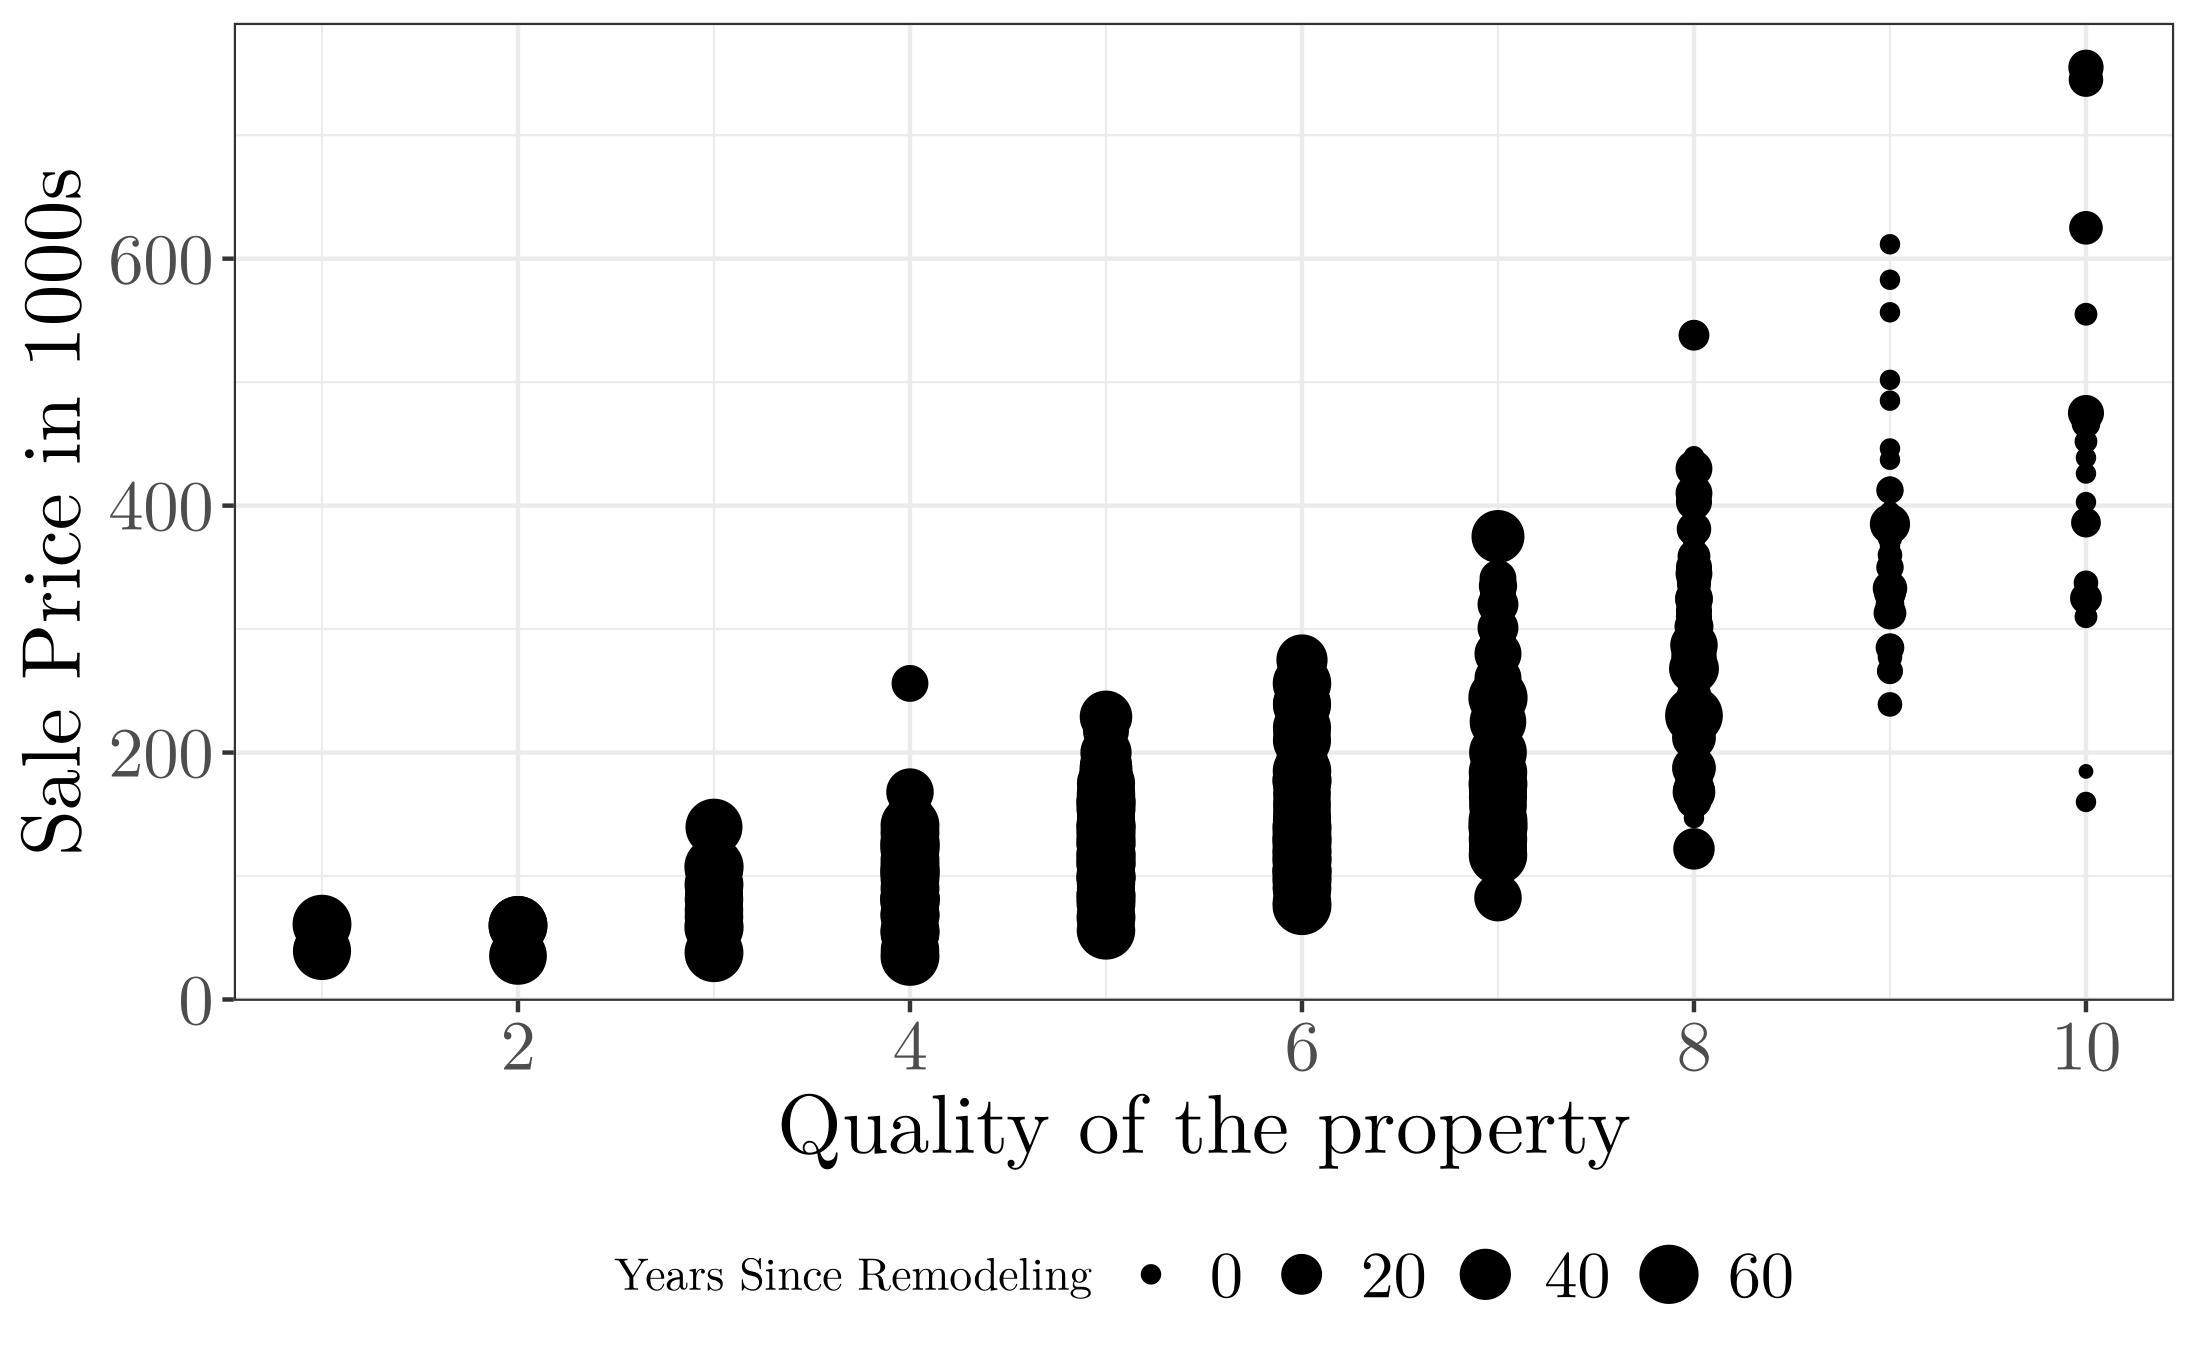
\includegraphics[scale=0.50]{"/home/angelo/Documents/Uni/Courses/Advanced Statistics and programming/Assignments/assignment1/Code/supplement_appendix_Quality_yearssinceremodeling_sale.jpg"}
         \small
         \caption{Quality of Property to Sales moderated by Years Since Remodelling}
\end{figure}





% Table created by stargazer v.5.2.3 by Marek Hlavac, Social Policy Institute. E-mail: marek.hlavac at gmail.com
% Date and time: Fri, Sep 16, 2022 - 16:20:11
\begin{table}[!htbp] \centering 
  \caption{Subset Analysis Regression} 
  \label{} 
\begin{tabular}{@{\extracolsep{0pt}}lcc} 
\\[-5.5ex]\hline 
\hline \\[-1.8ex] 
 & \multicolumn{2}{c}{\textit{Dependent variable:}} \\ 
\cline{2-3} 
\\[-1.8ex] & \multicolumn{2}{c}{SalePrice} \\ 
\\[-1.8ex] & Model (1) & Std.Coef\\ 
\hline \\[-1.8ex] 
 tot\_liv\_area & 0.033$^{***}$ & 0.338$^{***}$ \\ 
  & (0.004) & (0.004) \\ 
  & & \\ 
 y\_since\_rem & 1.890$^{***}$ & 0.491$^{***}$ \\ 
  & (0.231) & (0.231) \\ 
  & & \\ 
 low\_density\_zone & $-$1.610 & $-$0.008 \\ 
  & (9.192) & (9.192) \\ 
  & & \\ 
 commercial\_zone & $-$5.504 & $-$0.006 \\ 
  & (39.209) & (39.209) \\ 
  & & \\ 
 floating\_zone & $-$65.837$^{**}$ & $-$0.171$^{**}$ \\ 
  & (25.549) & (25.549) \\ 
  & & \\ 
 OverallQual & 31.370$^{***}$ & 0.546$^{***}$ \\ 
  & (1.322) & (1.322) \\ 
  & & \\ 
 y\_since\_rem:OverallQual & $-$0.418$^{***}$ & $-$0.564$^{***}$ \\ 
  & (0.040) & (0.040) \\ 
  & & \\ 
 tot\_liv\_area:low\_density\_zone & 0.009$^{**}$ & 0.155$^{**}$ \\ 
  & (0.004) & (0.004) \\ 
  & & \\ 
 tot\_liv\_area:commercial\_zone & $-$0.009 & $-$0.019 \\ 
  & (0.019) & (0.019) \\ 
  & & \\ 
 tot\_liv\_area:floating\_zone & 0.030$^{***}$ & 0.206$^{***}$ \\ 
  & (0.010) & (0.010) \\ 
  & & \\ 
 Constant & $-$104.441$^{***}$ &  \\ 
  & (11.037) & (11.037) \\ 
  & & \\ 
\hline \\[-1.8ex] 
R$^{2}$ & 0.779 & 0.779 \\ 
Adjusted R$^{2}$ & 0.777 & 0.777 \\ 
Residual Std. Error (df = 1449) & 37.489 & 37.489 \\ 
F Statistic (df = 10; 1449) & 510.275$^{***}$ & 510.275$^{***}$ \\ 
\hline 
\hline \\[-1.8ex] 
\textit{Note:} N = 1460 & \multicolumn{2}{r}{$^{*}$p$<$0.1; $^{**}$p$<$0.05; $^{***}$p$<$0.01} \\ 
\end{tabular} 
\end{table}








\end{document}
